\documentclass[10pt]{jarticle}
\usepackage{float}
\usepackage{adrobo_abst}
\usepackage[dvipdfmx]{graphicx}
\usepackage{bm}
\usepackage{amsmath, amssymb, amsfonts}
\usepackage[superscript]{cite}
\usepackage{enumerate}
\usepackage{url}
\usepackage{multicol}
\usepackage{mathtools}
%\usepackage[absolute]{textpos}

\renewcommand\citeform[1]{(#1)}

\begin{document}
    
    \makeatletter
    \doctype{2023年度卒業論文概要}
    \title{モデルの説明について}{(副題がある場合は括弧でくくる)}
    \etitle{Making Research Paper}{($\bigcirc\bigcirc\bigcirc$)}
    
    \author{20C1119\hspace{.5zw}森田大雅}
    \eauthor{Hiromasa Morita}
    
    \makeatother
    
    \maketitle
    
  
    \section{導\hspace{2zw}入}%==========================
	本研究に用いた座標系の記法やモデルのパラメータについて説明をする.
	図2の各パラメーは以下のことを示している.
	$l_n$はn番目リンク、$x_n, y_n, z_n$は座標系nのx軸、y軸、z軸、$\theta_n$はn番目のモータの回転角を表している.

	\section{手先の位置と回転角度の関係}
	図1に示すのは購入したooである. 
	このモデルの先端にペンを取り付け絵を描かせる.
	\begin{center}
	        \begin{figure}[!b]
	            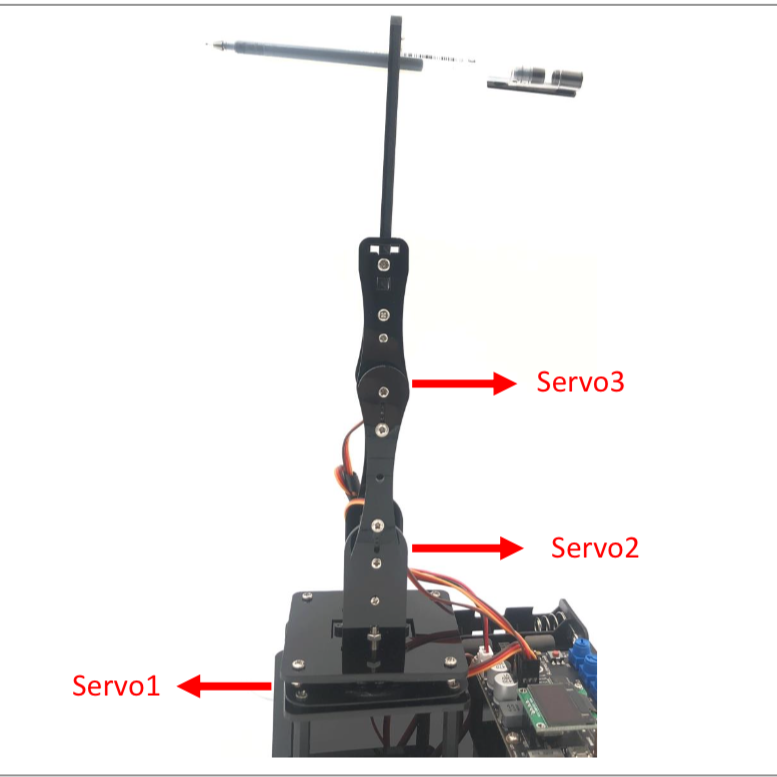
\includegraphics[width=0.45\textwidth]{/home/morita/ros2_ws/Memo/tex/img/IMG_0025.PNG}
    	        \caption{実機}
    	        \label{fig:sample-fig}
        	\end{figure}
    	\end{center}

3軸のロボットアームであるため、座標系を以下のように定義し、座標変換行列を用いて原点から手先までの位置を求める.
 \begin{center}
    	    \begin{figure}[!b]
            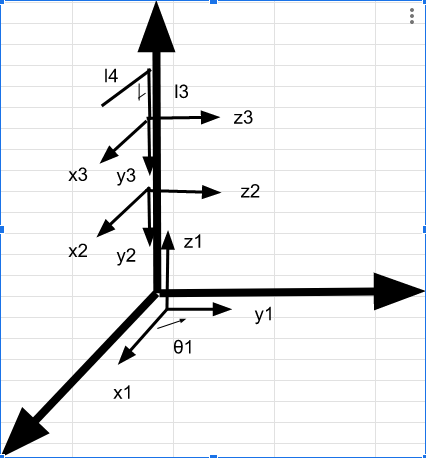
\includegraphics[width=0.45\textwidth]{/home/morita/ros2_ws/Memo/tex/img/link.png}
            \caption{リンク座標系}
            \label{fig:sample-fig}
        \end{figure}
    \end{center}


DH記法を用いて座標変換を行った結果、手先の位置x, y, zは以下のように求まる.
\begin{equation}
	\left\{
		\begin{array}{c}
		\begin{split}
			&x=C_1(l_4C_{23}+l_3S_{23}+l_2S_2) \\
			&y=S_1(l_4C_{23}+l_3S_{23}+l_2S_2) \\
			&z-l_1=-l_4S_{23}+l_3C_{23}+l_2C_2 \\
		\end{split}
	\end{array}
	\right.
\end{equation}
これらの逆運動学を解くと
\begin{equation*}
\left\{
	\begin{array}{c}
	\begin{split}
		&\theta_1=\frac{1}{2}cos^{-1}\biggl( \frac{x^2-y^2}{x^2+y^2} \biggr) \\
		\theta_2= cos^{-1}\biggl(& \frac{x^2+y^2+(z-l1)^2+l_2^2-l_3^2-l_4^2}{2l_2\sqrt{x^2+y^2+(z-l_1)^2}} \biggr)+\\
		&tan^{-1}\biggl( \frac{\sqrt{x^2+y^2}}{z-l1}\biggr) \\
		\theta_3=cos^{-1}\biggl(& \frac{x^2+y^2+(z-l1)^2-l_4^2-l_3^2-l_2^2}{2l_2\sqrt{l_3^2+l_4^2}}\biggr)+\\
		&tan^{-1}\biggl( \frac{-l_4}{l_3}\biggr)
	\end{split}
	\end{array}
\right.
\end{equation*}





\section{参考文献}

\begin{enumerate}
\item \lbrack 1\rbrack \ Raspberry Piを利用した肖像画描画ロボット :$ \lceil Pankraz Piktograph \rfloor$ \\
\item \lbrack 2\rbrack \ XDoG: An Xtended difference-of-Gaussians compendium \\
\item \lbrack 3\rbrack \ ロボットによる描画行為の再現\\
\item \lbrack 4\rbrack \ 出版:主婦の友社\ $\lceil \text{小河原智子の似顔絵入門} \rfloor$\\
\item 広瀬\ 茂男\ 著\ 機械工学選書\ 裳華房\ ロボット工学-機械システムのベクトル解析-\\
\item 細田\ 耕著\ 実践ロボット制御-基礎から動力学まで- \\
\end{enumerate}


\end{document}
